\documentclass[11pt]{article}
\usepackage[top=1in, bottom=1in, left=1in, right=1in]{geometry}
\usepackage{amsmath}
\usepackage{amssymb}
\usepackage{graphicx}
\usepackage{titlesec}
\titleformat{\subsection}[runin]{\normalfont\large\bfseries}{\thesubsection}{1em}{}

\begin{document}
\pagestyle{empty}
%\parindent=0pt

\section*{\centering Problem Set 11 (part 1)}

\section{Dust Temperatures and Opacity}
% XXX students did not like the length/insight ratio of this problem

The bulk of the interstellar radiation field in the Galaxy is from the light of
O stars, which have mass $\sim100M_\odot$.  There are $\sim5\times10^4$ O stars in the galaxy,
distributed over a cylindrical disk with radius 50 kpc and height 200 pc.

\subsection{}
Estimate the total energy density of starlight in the Galaxy in units of eV~cm$^{-3}$.
Use the fact that O stars radiate near the Eddington luminosity.

\subsection{}
This interstellar radiation field heats dust grains in the interstellar medium.
Estimate the temperature $T$ of the largest grains in the ISM, which have a radius
of $a\sim0.1$ microns.  Assume $Q_{abs}\sim1$ for wavelengths shorter than $2\pi a$,
and for longer wavelengths, take $m=1+0.25i$.
Is the grain hotter, cooler, or equal
to the temperature of an ideal blackbody placed in the interstellar radiation field.

\subsection{}
At what wavelength, $\lambda_{peak}$, does the energy density $(\nu F_\nu)$ of the grains peak?

\subsection{}
The largest grains carry most of the mass in the interstellar grain distribution.
Given a dust-to-gas ratio of $0.01$ and an average hydrogen number density
$n_H=0.1 {\rm cm}^{-1}$, calculate the specific intensity of the Milky Way
at $\lambda_{peak}$.

\subsection{}
Typically, the number density of dust grains scales with size as $dn/da\propto a^{-3.5}$ in
the ISM, where $dn$ is the number density of grains with radii between $a$ and $a+da$.  The
law holds over $a_{min}=10^{-3}$ microns to $a_{max}=0.1$ microns.  Plot the grain opacity
$\kappa(\lambda)$ contributed by all dust grains over the wavelength range $\lambda=0.1$ to
10 microns.  Consider only absorption and neglect scattering.  Indicate over each decade of
wavelength which grain sizes dominate the opacity.


\section{Diatomic}

\begin{figure}[!ht]\centering
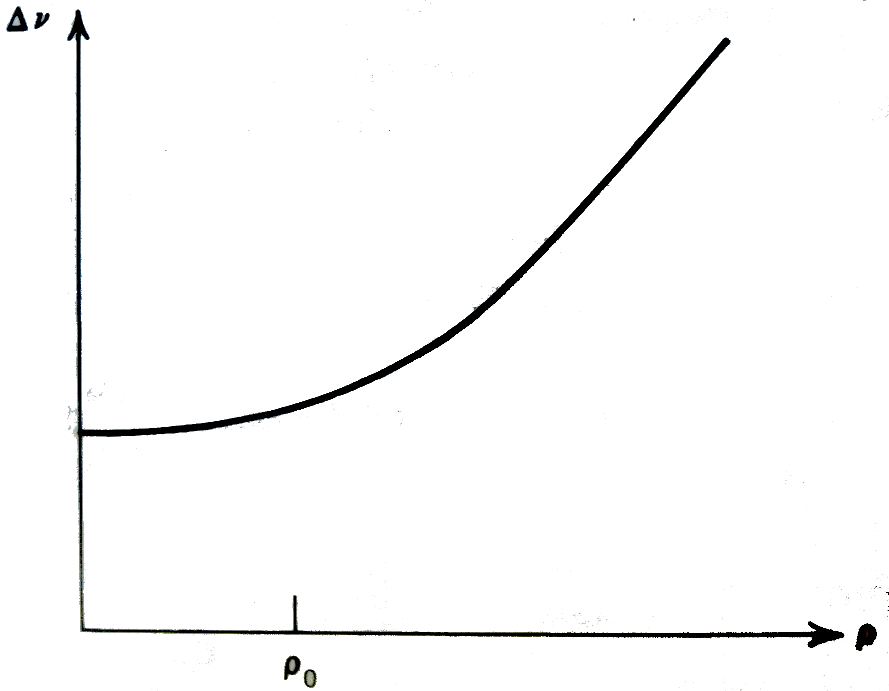
\includegraphics[width=2in]{ps11_linewidth.png}
\caption{
Line width as a function of density for emission from a medium of diatomic molecules.
}\label{fig:linewidth}
\end{figure}

Based on Rybicki \& Lightman 11.1.

Consider an electrically neutral medium of diatomic molecules in thermal equilibrium at
temperature $T$.  Each molecule contains one nucleus of mass $m_p$ and one of mass $2m_p$
at an equilibrium separation $r_0$.

\subsection{}
Estimate $r_0$ in terms of fundamental constants.

\subsection{}
Estimate the cross-section $\sigma_c$ for collisions between molecules.

\subsection{}

It is experimentally observed that , as a function of mass density $\rho$ of
the medium, the line width of the rotational lines has the form
shown in Figure \ref{fig:linewidth}.  If only Doppler and collisional broadening
are present, estimate $\rho_0$ and show that it may be written completely in
terms of fundamental constants, independent of $m_p$. 

\section{The Forest for the Trees}

\begin{figure}[!ht]\centering
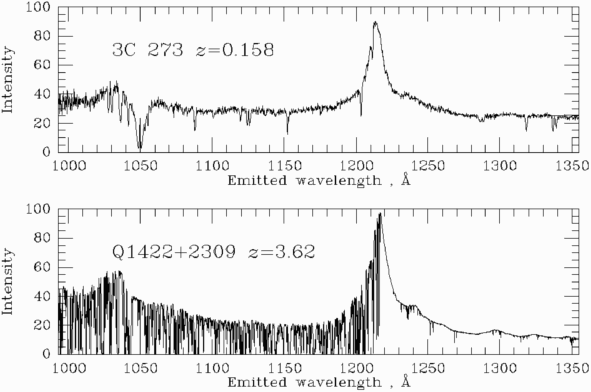
\includegraphics[width=3in]{lya_forest.png}
\caption{
Some typical Ly-$\alpha$ forest absorption features in high-redshift quasars.
}\label{fig:lya_forest}
\end{figure}

\subsection{}
Plot the Lorentzian (natural) line profile function for Ly-$\alpha$.  Overlay on the same plot a Doppler
profile corresponding to a temperature of 100 K.  Calculate numerically the total (Voigt) line profile
function and overlay it as well.  Make sure you get your normalizations correct.  Identify, in the Voigt
profile, the transition between the Lorentzian and Doppler-dominated regimes.

\subsection{}
Suppose we observe the Ly-$\alpha$ transition in absorption, perhaps because of a cloud of (fractionally neutral)
hydrogen backlit by a bright quasar.  Such clouds give rise to a ``forest" of absorption features in
high-redshift quasar spectra (which are typically called the ``Lyman-$\alpha$ forest") because redshifting
causes the Lyman-$\alpha$ frequency in the rest frame of the cloud to appear at different observed
frequencies (see Figure \ref{fig:lya_forest}).

Plot, for each of the line profiles above, the absorption feature
you would observe for a neutral hydrogen column density of $10^{16}~{\rm cm}^{-2}$.  You'll probably
want to think carefully about how to incorporate your line profile function into a cross-section for
absorption.

\subsection{}
If we were to measure the width (at half-max) of a particular ``tree" (absorption feature) in a
quasar spectrum, how could we back out the temperature and/or the column density of the cloud that gave
rise to that feature?  Over what range of optical depths might this be possible?  You may find it helpful
to tune your plotter over a range of column densities and temperatures to map out features that can help
you identify (and distinguish between) the observed effects of column density and cloud temperature.



\end{document}
